% ====================================================================
% background.tex (dissertation example)
% ====================================================================

\section{Background}
\label{sec:background}

\subsection{Quantisation error}

An ADC with a resolution of $N$ bits divides its input range into $2^N$ steps
of size $q$, and reports the step that the input falls in. The difference
between the true input and the centre of the reported step is the
quantisation error, and for an ideal converter it lies between $-q/2$ and
$+q/2$.

When the input moves across many steps between one sample and the next, the
error is close to being uniformly distributed over that range and unrelated
from sample to sample. Bennett showed that it can then be treated as noise
added to the signal~\cite{bennett_1948}, with a root-mean-square value of

\begin{equation}
  \label{eq:quantisationNoise}
  e_{\mathrm{rms}} = \frac{q}{\sqrt{12}}.
\end{equation}

Comparing this with the rms value of a full-scale sine wave gives the familiar
expression for the signal-to-noise ratio of an ideal
converter~\cite{kester_2005},

\begin{equation}
  \label{eq:snr}
  \mathrm{SNR} = 6.02N + 1.76~\unit{\decibel},
\end{equation}
which is \qty{74}{\decibel} for 12 bits. A real converter does a little worse
than this, and its performance is often quoted by working
\cref{eq:snr} backwards from the measured ratio to give an effective number of
bits (ENOB).

\subsection{Oversampling and averaging}

If $M$ readings are taken in the time that one was needed, and their errors
are unrelated to each other, the error in their average is smaller than the
error in a single reading by a factor of $\sqrt{M}$. This is the ordinary
result for the mean of independent measurements, and it applies to
quantisation error and to any other noise present, provided both are
unrelated from one sample to the next~\cite{oppenheim_schafer_2010}. If the
noise at the converter input has an rms value of $\sigma_n$, the error in the
averaged output is therefore

\begin{equation}
  \label{eq:averagedError}
  e_{\mathrm{out}} = \sqrt{\frac{q^2/12 + \sigma_n^2}{M}}.
\end{equation}

The number $M$ is the oversampling ratio (OSR). The arrangement is shown in
\cref{fig:oversamplingChain}.

% ====================================================================
% oversamplingChain.tex
% --------------------------------------------------------------------
% Block diagram of oversampling and averaging, drawn with plain TikZ.
% ====================================================================

\begin{figure}[htbp]
\centering
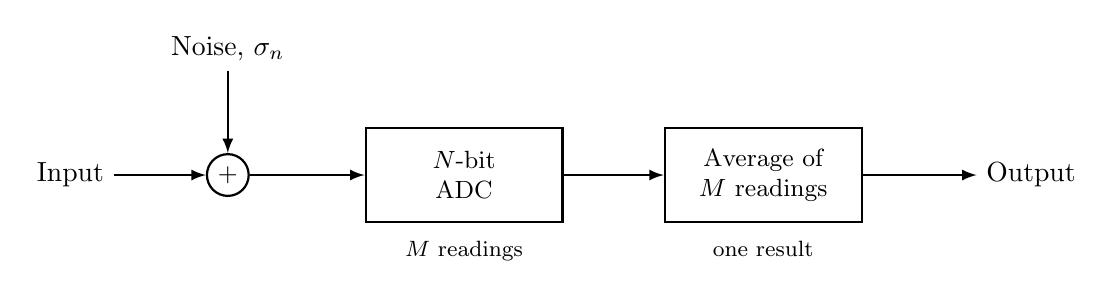
\begin{tikzpicture}[
  block/.style={draw, thick, minimum width=2.5cm, minimum height=1.2cm,
                align=center, font=\small},
  sum/.style={draw, thick, circle, inner sep=2pt, font=\small},
  >=latex
]
  \node (in) at (0,0) {Input};
  \node[sum]   (add) at (2.0,0)  {$+$};
  \node[block] (adc) at (5.0,0)  {$N$-bit\\ADC};
  \node[block] (avg) at (8.8,0)  {Average of\\$M$ readings};
  \node (out) at (12.2,0) {Output};
  \node (noise) at (2.0,1.6) {Noise, $\sigma_n$};

  \draw[->, thick] (in) -- (add);
  \draw[->, thick] (noise) -- (add);
  \draw[->, thick] (add) -- (adc);
  \draw[->, thick] (adc) -- (avg);
  \draw[->, thick] (avg) -- (out);

  \node[font=\footnotesize, below=3pt] at (adc.south) {$M$ readings};
  \node[font=\footnotesize, below=3pt] at (avg.south) {one result};
\end{tikzpicture}
\caption{Oversampling and averaging. The converter takes $M$ readings for
each output sample, and the output is their mean.}
\label{fig:oversamplingChain}
\end{figure}


Expressing \cref{eq:averagedError} as an effective number of bits, by
comparing it with the error of an ideal converter in
\cref{eq:quantisationNoise}, gives

\begin{equation}
  \label{eq:enobTheory}
  \mathrm{ENOB} = N - \tfrac{1}{2}\log_2\!\left(1 + \frac{12\sigma_n^2}{q^2}\right)
                  + \tfrac{1}{2}\log_2 M.
\end{equation}

The last term is the gain from oversampling, and it is half a bit for each
doubling of $M$, or one bit for each factor of four. The middle term is the
price of the noise, as noise that helps the averaging also adds to the error
that has to be averaged away. With $\sigma_n = q/2$ it is exactly one bit.
\Cref{eq:enobTheory} is the prediction that the simulation in this project
tests.

\subsection{The need for noise}

\Cref{eq:averagedError} relies on the errors being unrelated from sample to
sample. For a steady input and a noiseless converter this fails completely,
as every reading returns the same code and the same error. Widrow and
Koll\'ar give the formal conditions under which quantisation error behaves as
independent noise~\cite{widrow_kollar_2008}, and they are met when the input
to the quantiser varies by a step or more.

The practical guidance follows from this. The application note for one widely
used family of microcontrollers states that the signal must be oversampled by
a factor of four for each additional bit, and that the method relies on noise
of at least one LSB being present, which is to be added deliberately if the
circuit does not provide it~\cite{atmel_avr121_2005}. Added noise of this
kind is known as dither. What the guidance does not show is how the result
degrades as the noise falls below that level, or whether more noise than
necessary does any harm, and those are the questions the tests in
\cref{sec:method} were designed to answer.
